%\documentclass[a4paper,10pt]{article}
\documentclass[sigconf, anonymous, pdftex]{acmart}
%\usepackage[utf8]{inputenc}

%\usepackage[]{tikz}

%% \usepackage[backend=bibtex,
%% style=numeric,
%% bibencoding=ascii
%% %style=alphabetic
%%  %style=reading
%% ]{b
%  iblatex}

\usepackage{graphicx}
\usepackage{array}
%\addbibresource{Bibliography.bib}

\title{Bibliography management: \texttt{biblatex} package}

\title{An Approximation Approach to a Weighted Variation of the TSP}
\author{Tanner Bina, Alec Justice, Joseph Mugisha, and Douglas Szajda}
\date{June 2017}

\begin{document}

\maketitle

\section{Abstract}

The Traveling Salesman Problem (TSP) has been studied extensively for years due to both its applications and complexity, leading to the development of many near optimal heuristic approaches. We present a new variation of this problem, the Tennis Ball Collector Problem (TBCP), in which travel costs increase based on tour position. This new problem has both real world applications and is interesting in the field of computational complexity as it increases the TSP's hardness by using a varying cost matrix. We present a novel approximation algorithm that deploys clustering, branch and bound, and the divide and conquer paradigm to quickly approximate large instances of the TBCP. To demonstrate the efficiency of this algorithm, we test it against other common heuristical methods to solve TSP Variations. Our approximation algorithm not only provides good scaling and solutions, but also allows for further improvements as the study advances.

\section{Introduction}

The Traveling Salesman Problem (TSP) is a problem that falls into the designation of NP-complete problems. NP-complete problems are some of the hardest problems in computing as they cannot be solved by deterministic algorithms in polynomial time despite being solvable by non-deterministic algorithms in polynomial time \cite{pVsNp}. The problem statement of the TSP asks if a Hamiltonian cycle exists with a total cost less than a budget, $b$, over a directed weighted graph; however, we make a more difficult specification for the TSP in which the cycle found must be the lowest cost cycle possible \cite{tspAll}. Due to the difficulty of finding exact solutions for the TSP, many method have been developed to approximate such solutions as a good approximation is usually all that is necessary\cite{approximateTSP}.


Alongside the study of the Traveling Salesman problem, many variations have been studied such as the time-dependent traveling salesman problem\cite{tdtspDefinition}\cite{tspAll}. These variations are studied for both their practical applications as well as the academic significance as difficult problems. Many of these variations become more difficult as common heuristic practices for the TSP are ineffective for solving these problems.

In our paper, we present a new variation of the TSP, the Tennis Ball Collector Problem (TBCP). The TBCP attempts to find the lowest amount of work, based on a cost matrix, required to visit a set of vertexes on a x,y Euclidean coordinate plane. In the TBCP, the cost of visiting a vertex depends upon the number of vertexes visited prior. The cost increases by a uniform multiplier based on the number of vertexes visited. This variation has many applications in real world scenarios as well as being computationally interesting due to the changing cost matrix for visiting vertexes. Our paper presents a new approximation algorithm for this variation which allows large instances to be approximated as well as a new branch and bound method for finding exact solutions for small vertex sets. We then compare our algorithm results to commonly used TSP heuristic algorithms to evaluate our results.

\section{Related Work}

The Traveling Salesman Problem was first formulated in 1930s by mathematician Karl Menger \cite{tspHistory}. Originally arising in connection to a proposed new definition for curve length, the TSP became a widely studied problem due to its NP-complete designation \cite{pVsNp}. It is widely studied due to both it's practical applications and its relevance to other NP-complete and combinatorial optimization problem \cite{tspAll}. Throughout the course of the problems study, many attempts were made to find exact solutions to the problem. The most successful of these taking advantage of branch and bound principles \cite{bbAlgorithmsGeneral}\cite{branch&boundBasics}\cite{branchBoundTSP}; however, branch and bound algorithms could only find the optimal for small instances of the TSP. This led to the development of heuristic algorithms \cite{tspAlgorithms}\cite{approximateTSP}. These algorithms attempted to find a near optimal solution for large instances of the traveling salesman problem in polynomial time. One of the most successful and widely used heuristic algorithms, the Lin-Kernighan heuristic, was developed in 1973 \cite{lkHeuristic}. Using variations of this alongside a clustering mechanism problems of up to one million vertexes could be approximated \cite{dcClusteringMillionTSP}.

As the study of the TSP advanced, many variations with more specific conditions and constraints arose \cite{tspAll}. Most of these involved varying the cost matrix of the TSP in various ways, with one of the most widely studied variations being the Time Dependent Traveling Salesman Problem \cite{tdtspDefinition}. In this variation, the cost matrix varies based on the position in which it is traveled. Similar to the original TSP, many different types of algorithms have been developed for this variation \cite{tdtspOptimalGenerator}\cite{dpTDTSP}.

In this paper, we present the Tennis Ball Collector Problem, a new variation of the TSP which can be seen as a sub-problem of the TDTSP. We develop a branch and bound algorithm inspired by the lower bounding procedure developed in \cite{bbTardyMachine} as well as common branch and bound techniques \cite{branch&boundBasics}. Using this branch and bound algorithm, we attempt to tackle large scale instances. Various other algorithms have used the method of clustering and divide and conquer to approximate instances of both the TDPTSP and TSP \cite{dcClusteringMillionTSP}\cite{GAclusterTSP}\cite{tspLargeClustering}. We draw inspiration from these developed techniques and expand their uses to our specific variation of the problem.


\section{Problem Statement}

Our problem is the Tennis Ball Collector Problem. From a high level, the problem asks what the most efficient way is for one person to move around two dimensional euclidean plane and collect n tennis balls, given that collecting a tennis ball makes it more difficult to visit the next tennis ball. The collector then must return to the starting location once all balls are collected. The problem is a direct variation of the TSP where instead of minimizing distance traveled the goal is to minimize work done over a tour. The problem can also be seen as a variation of the Time Dependent Traveling Salesman Problem in which travel time increases at a uniform weight with position.

An instance of a TBCP includes a start vertex, $S$, end vertex, $E$, vertexes to be traveled through $V$, and a uniform weight $w$. The goal is to find the tour which optimizes the amount of work done where work is a calculation based off the number of balls visited prior and the distance traveled to visit the next ball. An optimal tour must meet the criteria given for any TSP variation problem such as subtour elimination and continuity.

The constraints of an optimal tour are the same as the constraints given in most Time Dependent Traveling Salesman Problems \cite{tdtspDefinition}. The calculation for the minimization, however, changes due to the cost matrix being only two dimensional and position being a relevant factor. This alteration allows for many heuristics to be used for the TBCP that are not applicable for the TDTSP. We leverage one of these, a heuristic clustering mechanism, as the driving point for our algorithm.

Although many algorithms have been developed that can find an optimal or near optimal solution to the TSP in polynomial time, these algorithms fail at finding efficient solutions for the TBCP. This is due to the failure of many common TSP heuristics such as nearest neighbor searches and cross elimination. Although more difficult than the TSP, the TBCP does allow for some heuristics due to the linearly increasing nature of the cost matrix. One such heuristic that we leverage in our algorithm to obtain solutions is the ability to use clustering as a divide and conquer mechanism. This mechanism has previously been shown to be efficient but requires adaption to be useful for the TBCP \cite{dcClusteringMillionTSP}\cite{tspLargeClustering}.

We propose in the next section an algorithm that can approximate quickly and effectively large instances of the TBCP. Small instances can be solved optimally using the branch and bound subsection of our algorithm presented, but as with most branch and bound algorithms, the runtime becomes large when problem sizes move over $30$ vertexes. The algorithm presented can run quickly on problems ranging from $30$ vertexes to $10,000$. The structure of the algorithm is also very applicable to parallel processing and could solve extremely large instances of the TBCP if parts were ran in parallel. 

\section{Algorithm Overview}

The proposed algorithm attempts to quickly find an approximate solution for the TBCP using branch and bound, clustering, and the divide and conquer paradigm. The first part of the algorithm leverages parts of well defined clustering algorithms to break the problem into smaller subproblems \cite{clusteringAlgorithms}. The smaller problems can be placed into a correct order by determining the optimal tour over the clusters found themselves. This is done in a similar manner as used in \cite{tspLargeClustering}. Using this order, these problems become true subproblems with defined start and end points. Each subproblem is continually reduced until the optimal solution of a subproblem can be efficiently found using branch and bound. Once the optimal solution to all subproblems is found, the subproblems are recombined in the order found through the original clusters. The recombination and subsequent optimization of these subproblems produces the final tour.

In the next subsection we will define the main method calls, parameters, and classes used in the construction of the algorithm. Afterwards we will go through the execution of the three main sections of the algorithm, Divide and Conquer, Clustering, and Branch and Bound.

\subsection{Definitions}

Here we will define the terms used within the algorithm, including any predefined parameters and the main method calls.

\begin{enumerate}
    \item $CUT :=$ A predefined variable which determines the maximum number of nodes that the algorithm should attempt to optimally solve using branch and bound. Set to $20$ through experimental analysis.
    
    \item $TMAX :=$ A predefined variable which determines the maximum amount of time the algorithm should spend attempting to reach the optimal branch and bound solution. The value should be set to high enough that only extreme circumstances of instances of size $CUT$ do not solve within the time. Set to $3$ seconds through experimental analysis on point sets of size $20$ (Fig. 1).\footnote{It should be noted that the values of $TMAX$ and $CUT$ are relative to one another. Higher $CUT$ values should be paired with higher $TMAX$ values and may increase time and performance. Based on the system and application in which the algorithm is used, they could be tweaked to increase performance or decrease runtime.}
    
    \item $Vertex :=$ A vertex within the TBCP instance. It contains the $x$ and $y$ euclidean mapping of the vertex onto a plane. It also contains a $z$ coordinate that is defined by the distance from this point to the centroid of the cluster that it is in. As this is not an innate characteristic of the point, it is set during the execution of the algorithm.
    
    \item $Cluster :=$ A set of vertexes which holds additional information about them. It contains a unique ID, the set of vertexes within the cluster, the length of the minimum spanning tree of all points within the cluster and the cluster's centroid. The centroid of the cluster is an abstract vertex which has the average x, y, z coordinates of all vertexes within the cluster, a weight equal to the number of vertexes within the cluster, as well as an additional property referred to as $VDIST$. $VDIST$ is set to the distance obtained for the minimum spanning tree of the cluster and is used for some instances of branch and bound used within the algorithm.
    
    \item $Tour :=$ A tour which consists of a start vertex, $s$, end vertex, $e$, an ordered list of vertexes, $\phi$, as well as a value for work, $w$ defined by the problem statement.
    
     \item $BBNode(C, R, S) :=$ A branch and bound node. The node is constructed by inputting the constraining partial tour $C$, remaining vertexes to be visited $R$, as well as the starting vertex of the problem $S$. When a $BBNode$ is created, the lower bound is immediately found.
    
    \item $TwoOpt(T) :=$ The method header for a call to two step optimization for an inputted tour $T$. Returns the optimized tour.
    
    \item $InsertOpt(T) :=$ The method header for a call to insert optimization for an inputted tour $T$. Returns the optimized tour.
    
    \item $ClosestVertex(C_1, C_2) :=$ The method header for a call to find the closest vertex within $C_2$ to any vertex in $C_1$.
    
    \item $SizeMST(V) :=$ The method header for a call to find the distance of a minimum spanning tree over the vertexes in $V$.
    
    \item $Optimal(S, E, V, SW) :=$ The method header for a call to a brute force solver for a TBCP instance. The brute force solver works on TBCP problems as well a centroid TBCP where a value of $VDIST$ and variable weights are defined. The inputs are a start vertex, end vertex, every vertex to be visited, and the start weight of the tour. The method returns the optimal tour.
    
    \item $BranchBound(S, E, V, SW) :=$ The method header for a call to branch and bound. The inputted values are $S :=$ the starting vertex, $E :=$ the ending vertex, $V :=$ the set of vertexes which should be traveled through to reach $E$, and $SW :=$ the starting weight of the branch and bound instance.\footnote{This value is used during the algorithm as branch and bound calls are made for various sub problems. These subproblems will occupy different sections are the final tour, thus having differing start weights which must be accounted for in finding the optimal solution.} The branch and bound algorithm runs until the optimal solution is found or until the elapsed time surpassed $TMAX$. It returns the optimal tour or the best tour found so far accordingly.
    
    \item $Cluster(V) :=$ The method header for a call to cluster a set of vertexes. The method takes in the vertexes that should be clustered. It returns a set of clusters of size $CUT$.
    
    \item $DivideConquer(S, E, V, SW) :=$ The method header for the recursive algorithm. It takes in a start vertex, end vertex, list of vertexes to be traveled over, and a start weight respectively. Returns a tour. The algorithm makes recursive calls on itself as well as calls to cluster and branch and bound on the inputted vertexes to produce the returning tour.\footnote{Note that this is the main part of the algorithm and the call which begins its execution.}
    
    
\end{enumerate}

    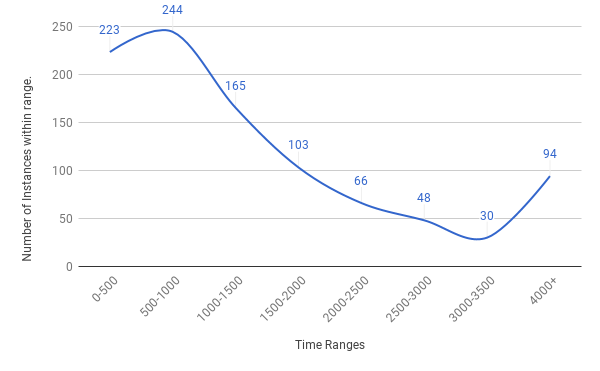
\includegraphics[scale=.38]{bbTime}
    
    Fig 1. Time range of 1000 branch and bound runs of size 20 point sets using randomized C-TBCP\footnote{A C-TBCP instance uses variable weight values for vertexes as well as VDIST values. The definition for this variation is in Section 5.4}. As almost $\%90$ of the branch and bound instances find the optimal within 3 seconds, the value of $TMAX$ is set to 3 seconds to maximize the number of optimal tours found while minimizing overflow time.

\subsection{DivideConquer}

The DivideConquer method is the heart of our algorithm. Using the divide and conquer paradigm, it recursively reduces TBCP problems until they are solvable. The algorithm uses both $Cluster$ and $BranchBound$ to achieve this as well as the optimization methods, TwoOpt and InsertOpt.\\

$DivideConquer(S, E, V, SW)$\\

As in all recursive algorithms, the initial step of DivideConquer is to check the base case. The base case is if $sizeOf(V) \leq CUT$. This is because if the number of inputted vertices is less than the value of $CUT$, the vertices can be branch and bounded over to obtain an optimal or near optimal solution.\footnote{Note that this is only if the value of $CUT$ corresponds to the value of $TMAX$. If they do not correspond, the solution may not be near optimal.} If the base case is met, then the result of the call $BranchBound(S, E, V, SW)$ is returned.

If the base case has not been met, the problem must further be broken down and reduced. A call to $C = Cluster(V)$ is made using the inputted vertexes of DivideConquer, $V$. By definition of $Cluster(V)$, $|C| = CUT$. The centroid of each cluster within $C$ is then converted into a vertex. As these vertexes are derived from cluster centroids, the value of $VDIST$ is carried over to the corresponding vertex and used in further execution of the algorithm. These vertexes are used to form the list of vertexes $Cents$. A call is then made to find the optimal order of $Cents$, which will be used as the order in which each cluster should be visited and the formation of the recursive calls.

The optimal tour of the centroids, $T_{Cents}$, is found through $T = BranchBound(S, E, Cents, SW)$. Since each centroid within $Cent$ corresponds to a cluster within $C$, $C$ is then sorted based on the order of visitation found in $T_{Cents}$. This ensures that the recursive calls happen in the optimal order.

The recursive calls find approximate tours of the subproblems which form naturally over the vertexes within each cluster. They are solved in the order determined by the ordering of $C$. For $C_1 \dots C_{CUT}$, a recursive call is made and the results are stored in a list of tours $T$. The recursive call for $C_i$ is as follows :

$S_i = ClosestVertex(C_i, C_{i-1}) : $ if $i = 1, S_i = S$

$E_i = ClosestVertex(C_i, C_{i+1}) : $ if $i = CUT, E_i = E$

$SW_i = \Sigma_{j=1}^{i-1} |C_j|$

$T_i = DivideConquer(S_i, E_i, C_i.Vertexes, SW_i)$

Once $T_i : 1 \leq i \leq CUT$ is defined, the recombination process can start. To begin, for every value of $T_i$, the points $S_i$ and $E_i$ are removed to avoid duplicate visits of these points in the final tour. These newly edited tours will be referred to as $T_i^*$. We then construct an empty tour, $T_{Final}$. The vertex $S$ inputted into the original call of DivideConquer is placed into the first spot of $T_{Final}$. The modified tours are then concatenated onto the final tour in their sorted order $T_{Final} = T_{Final} || T_i^* : 1 \leq i < CUT$. Finally, $E$ is concatenated with $T_{Final}$ to produce a tour starting at $S$, ending at $E$, and visiting every vertex within $V$.

The last step before returning $T_{Final}$ is to optimize the tour to its local minimum. This is done by making a call to $InsertOpt(T_{Final})$, followed by a call to $TwoOpt(T_{Final})$. $InsertOpt$ is called first as it can make more dramatic changes to the tour than $TwoOpt$ and can reach a deeper optimization level. The call of $TwoOpt$ reaches the true local minimum of the edited tour. Finally, $T_{Final}$ is returned as the method result in its optimized form.

\subsubsection{TwoOpt}

Two Opt is a common optimization method for TSP problems and their variations. The optimization works by attempting to switch the ordering of two points. Given the order $v_1 \dots v_{i-1}, v_i, v_{i+1} \dots v_{j-1}, v_j, v_{j+1} \dots v_n$, the algorithm determines if the work of $v_1 \dots v_{i-1}, v_j, v_{i+1} \dots v_{j-1}, v_i, v_{j+1} \dots v_n$ is less than the previous work for every $1 < i < n, 1 < j < n, i \neq j$. It is a constant time operation to determine the change of work, whereas the loops run in $n^2$ time.

The actual Two Opt algorithm iterates multiple times as continual improvements are possible. Our algorithm continually runs two opt until the work improvement of a run is less than $.1\%$ of the original work. At this point, the algorithm terminates as a point near the local minimum has been reached.

\subsubsection{InsertOpt}

Insert Opt is a new optimization method which has produced significant results for the TBCP. The optimization works by attempting to insert a specific point into a different position in the tour. Given the order $v_1 \dots v_{i-1}, v_i, v_{i+1} \dots v_{j-1}, v_j, v_{j+1}\\ \dots v_n$, the algorithm determines if the work of $v_1 \dots v_{i-1}, v_j, v_i,\\ v_{i+1} \dots v_{j-1}, v_{j+1} \dots v_n$ is less than the previous work for every $1 < i < n, 1 < j < n, i \neq j$. It is a constant time operation to determine the change of work, whereas the loops run in $n^2$ time.

The actual Insert Opt algorithm iterates multiple times as continual improvements are possible. Our algorithm continually runs insert opt until the work improvement of a run is less than $.1\%$ of the original work. At this point, the algorithm terminates as a point near the local minimum has been reached.

\subsection{Cluster}

The Cluster method is vital to the efficiency of the algorithm as it allows the problem size to be reduced as well as allowing the general order of the vertexes to be found. A large amount of the algorithm's accuracy is determined by the clustering. If the clustering algorithm can optimally cluster the vertexes for a TBCP, our algorithm can produce the optimal solution. This is due to the innate fact that any partial optimal tour of a TSP, and from extension TBCP, is an optimal tour itself. For example, let $\phi$ be the optimal tour, where $\phi = S, v_1 \dots v_{i-1}, v_i \dots E$, with $S$ being the start point and $E$ the end point. The partial tour $\phi^* = S, v_1 \dots v_{i-1}, v_i$ is then itself an optimal tour from $S$ to $v_i$, going through the points $v_1 \dots V_{i-1}$. Since the algorithm determines optimal cluster visit order as well as optimal base case order, if the clustering has optimally determined which vertexes are $v_1 \dots v_{i-1}$, the algorithm will be able to find the optimal tour for the whole problem. The clustering algorithm draws inspiration from hierarchical clustering algorithms discussed in \cite{clusteringAlgorithms}.\\

$Cluster(V)$\\

The cluster algorithm takes in a list of vertexes, $V = \{ v_1 \dots v_n \}$, and returns a list of clusters $C = \{ c_1 \dots c_|CUT| \}$. The basis of the clustering algorithm being used is a hierarchical clustering over 3 dimensions of each vertex. This is completed by using three dimensional centroids. A centroid is a vertex with the average x, y, and z, coordinates of a list of vertexes, $Verts$. The weight of a centroid is the number of vertexes in $Verts$. As well as this, the centroid contains a value for $VDIST = SizeMST(Verts)$. The first two dimensions of the vertexes are their $x$ and $y$ coordinates. The third dimension is a $z$ dimension. This is calculated immediately for every vertex by calculating a centroid over all points, $V$, using only the $x$ and $y$ dimensions as the $z$ dimension is still undefined. Let us refer to this centroid as $Cent_{all}$. The $z$ for a particular vertex, $v_i$, is then $v_i.z = distXY(v_i, Cent_{all})$.

The $z$ distance is used to attempt to increase the clustering of outliers together into their own clusters. Many TBCP tours involve visiting outlying clusters at the beginning of the tour as to travel these longer distances prior to picking up large amounts of weight. Using the $z$ dimension has shown to increase the accuracy of generating tours compared to the accuracy of generating tours using only the $x$ and $y$ coordinates.

Once the $z$ value is set for all vertexes, the main clustering loop can begin. The first step creates the original list of $C$, in which every vertex is its own cluster.\footnote{As soon as a cluster is created or edited its Centroid is calculated.} The loop then calculates the distance between all clusters using $d_{i,j} = distXYZ(Cent_i, Cent_j)$. The minimum value is then taken, where the minimum values are $i$ and $j$. The two clusters $C_i$ and $C_j$ are combined, whereas $V_{C_i} \cup V_{C_j}$, and the centroid of the new cluster is calculated. This loop continues until there are $CUT$ clusters left in $C$. The list of clusters $C$ is then returned as the result of the clustering. 

\subsection{BranchBound}
To find the optimal tour to subproblems as well as optimal tours through clusters, we use a new Branch and Bound algorithm. These tours are essential as they determine the overall visit order of clusters as well as the base case optimal tour of clusters. Our algorithm uses a basic heuristic algorithm to determine the upper bound and a new approach to finding the lower bound building on the methods developed for lower bound derivation with respect to the general TSP problem \cite{TravelingMST}. \\

$BranchBound(S, E, V, SW)$\\

The inputs for the branch and bound algorithm are a start vertex, end vertex, vertexes to travel through and starting weight, respectively. The branch and bound algorithm automatically terminates if at any point the elapsed time surmounts the value of $TMAX$\footnote{This should be a very rare case if $CUT$ is set properly as premature termination leads to inefficient tours.}. If the algorithm terminates early, the best found tour so far is returned. The algorithm is guaranteed when supplied with enough time to find the optimal TBCP solutions over $V$. The algorithm works by constructing nodes of the solution space tree, a tree in which each node represents a partial tour in the solution space. Each node has a represented constraint, $C$, which allows for the determination of the lower bound. The branch and bound algorithm cuts any node which has a lower bound value greater than the current upper bound. Using a lowest bound branching strategy, the algorithm explores the lowest lower bound value of each node until a complete tour can be made with $C$. This tour is then set as the new upper bound if it has a lower work value than the current upper bound. The algorithm follows this strategy for every node until the full tree has been explored, at which point the upper bound tour is the optimal tour.

The branch and bound algorithm we present is built to work on vertexes that are both from TBCP problems as well as vertexes which are centroids. Vertexes which are centroids can have varying values of their weight as well as contain a value for $VDIST$. For this reason, in our algorithm, we refer to the weight of vertexes, $v.w$, as well as the $VDIST$, $v.VDIST$. It should be noted for any inputted TBCP problems $v.w = 1$ and $v.VDIST = 0$. With these values set, the branch and bound algorithm will produce the optimal solution for TBCP problems. When these values vary, the algorithm will produce the optimal solution for a Centroid specific TBCP, (C-TBCP) problem. 

\subsubsection{Upper Bound Derivation}

The original upper bound is derived from a fast heuristic algorithm whose resulting tour is then optimized using both Insert Opt and Two Opt. The heuristic attempts to minimize the cost of traveling to a vertex as well as the expected increase of cost for visiting that vertex in the position it is visited in. These estimations are made in a similar way as the lower bounding process which will be covered later; however, the tour generated will always be a valid tour.

The first step of algorithm is to find the minimum spanning tree, $T$, and the total edge weight of the MST. This is used to approximate the increase of future cost for visiting a vertex. The algorithm then begins a nearest neighbor process for determining which vertex to visit next. The nearest neighbor formula is slightly modified so that the nearness of a neighbor is measured by $nearness_{i, j} = currentWeight * dist_{i, j} + (currentWeight + v_i.w) * mstDist$. The first part of the formula is calculating the work to visit the vertex, whereas the second part calculated the increase of work for traveling the rest of the MST with the increased weight. Once the nearest neighbor is chosen and added onto the partial tour, the maximum weight edge that includes the nearest neighbor vertex is found. The weight of this edge is then removed from the MST distance. After all vertexes are added to the tour, the tour is optimized with insert opt and two opt.

\subsubsection{Branching Strategy}

The branch and bound algorithm uses a constraining partial tour $C$ to determine the lower bound and define distinct nodes within the branch and bound tree. The partial tour $C$ is a set of vertexes so that $C = \{v_i \dots v_j, E\}$, where $E$ is the end point inputted into the branch and bound algorithm and $v_i \dots v_j \in V$. This partial tour determines the end visitation order of all tours generated by children of that node. One child is created for each vertex in the remaining vertexes to be visited, $R = r_1 \dots r_k$, where this vertex is appended to the front of the new $C$ for the given child. This creates every possible permutation with the ending sequence given by $C$.

The purpose of defining the optimal tour from the end vertex to the start vertex rather than the commonly used reverse way is to maintain the highest possible lower bound for each node. This idea was proposed in \cite{bbTardyMachine} and showed much more effective results for problems of this nature. Since the cost of travel increases based on the number of nodes visited and the weight acquired while visiting previous nodes, the edges with the highest costs are the final visits. For this reason, building a tour from the back forward defines these high cost edges quickly, which forces the upper bound to be greater and allows the early pruning of in-optimal nodes.

The root of the branch and bound tree is defined by a $C$ consisting only of the end vertex, $E$. The remaining vertexes to be visited, $R$, consists of all the inputted vertexes in $V$. Therefore, we can define $root = BBNode(\{E\}, V, S)$. When a node is created, the lower bound is immediately determined. Then, a call is made to $root.explore()$. Exploring a node is a recursive method which explores all subtrees of the node which have a lowerbound less than the current upper bound. We will define the implementation of the explore method next as once $root.explore()$ is executed, the recursion will fill in the tree and set the upper bound to the optimal solution. This optimal solution is then returned.

The explore call can be made on any node. The first step is to check if the current node is completed or not. A completed node can be defined as one in which $|R| = 0$ and every $v \in V$ is $\in C$ as well. If a node is completed, start vertex $S$ is appended to the front of the list $C$. $C$ can then be considered the tour $T_C$. The work of $T_C$ is then compared to the current upper bound. If it is less than the current upper bound tour's work, $T_C$ is set as the new upper bound. The algorithm returns upon checking this, completing the explore call.

If the node is not a complete node, the children are created for the node. For each vertex in $R$, the algorithm attempts to create a child of the current node, so that it can be insured that every permutation ending in $C$ is accounted for. The new value of $C$ for each child is calculated, where $C_i = r_i \cup C$ and $r_i \in R$. Corresponding to each of these is a value for $R_i = R/r_i$. The algorithm then checks if  $C_i$ is the optimal constraint, for each value of $i$. This can be done by generating the tour $T_i = Optimal(r_i, C/E, E, \Sigma_{j=0}^{|R|}r_j.w)$. If the order of $T_i$ is equal to $C_i$, then $C_i$ represents the optimal constraint. If $C_i$ is not the optimal constraint, the child corresponding to it can be cut, because an optimal tour is made up of optimal subtours as explained previously. This process only occurs if the size of $C_i$ is less than $6$. This is because determining if a large constraint is optimal is computationally expensive and pruning a node with a large constraint does not provide a large benefit as there are few remaining permutations within that subtree.

Once all children have been created whose constraints are optimal, they are then sorted based on the lower bound values, which are determined automatically. A call is then made to explore each child in order, if the childs lower bound value is less than the current upper bound. If the lower bound is greater than the upper bound, the child is cut. Once every child has been explored, the explore call terminates. 

\subsubsection{Lower Bound Determination}

Whenever a new branch and bound node is created, the lower bound must be determined. This lower bound is dependent on the constraining partial tour $C$. The lower bound is determined by relaxing some of the constraints of a $C-TBCP$ so that it can be solved in polynomial time. The $C-TBCP$ travels from the starting vertex of the node $S$ through all the remaining vertexes in the node $R$, and ends at the first vertex in the node constraint $C_1$. The relaxation allows for edges to be traveled without visiting their start vertexes as well as allows vertexes to has a degree greater than two in the final tour. For example, $v_i$ does not have to be visited before an arbitrary position $k$ in the tour, for the edge $v_i \rightarrow v_j$ to be traveled at position $k$ in the tour. The second relaxation allows the edges $e_{v_i, v_j}$ and $e_{v_i, v_l}$ to exist in the final solution to the problem. This relaxed problem will be referred to as the $C-TBCP^R$.

The $C-TBCP^R$ can be solved in polynomial time through an algorithm that uses the edges of the minimum spanning tree of the vertexes. As the edges of a minimum spanning tree are by definition the shortest edges, an optimal solution will contain only those edges as replacing one edge in the solution with an edge not in the MST would result in a tour with a higher value for the work calculation. The problem then is simplified for finding the optimal $k$ values for each of the edges in the minimum spanning tree. This can be done through a bound determining algorithm.

First, the algorithm finds the MST over all vertexes $R \cup S$ as these are the edges for which $k$ values must be found\footnote{The reason $E$ is not included in the MST is that the $k$ value of whatever edge ends at $E$ is already set by constraint $(16)$}. Three values are determined after the MST is found. The first, $MST_{Dist}$, is the summed distance of all the edges of the MST. The second value, $VDIST_{Left}$, is the sum of the $VDIST$ values for all the vertexes in $R$. These two values will be used in determining the bounds of each edge as they represent how much an increase of weight will increase the amount of work to be done to complete the rest of the tour. The third value is $W_{current} = SW$, which keeps track of the current weight in the tour. The solution $\phi$ is then declared as an empty edge set that represents the solution to the $C-TBCP^R$. The next step is to determine the dependent vertex of each edge in the minimum spanning tree. We define the dependent vertex for an edge, $e$, as the vertex which is no longer connected to $S$ with edges in the MST after removal of $e$ from the minimum spanning tree. This vertex will be referred to as $e_{dep}$ from now on for each $e$.

The algorithm then enters a loop in which the order of each edge in the MST is determined. The loop first calculates the edge with the minimum bound, $e_{min}$ with the following calculation $e_{min} = Min \{ W_{current} * (e.dist + e_{dep}.VDIST) + (e_{dep}.w + W_{current}) * (MST_{Dist} - e.dist + VDIST_{Left} - e_{dep}.VDIST : e \in MST \}$. Although this bound calculation looks overwhelming at first, it can be broken down into two distinct logical parts for an edge $e$. The first part is determining the amount of work which will be required to travel this edge. That can be found by multiplying the current weight by the distance of the edge plus the value of $VDIST$ associated with the dependent edge. This is the work calculation used in the definition of the $C-TBCP$ for visiting a vertex at some point in the tour. The second part of the bound is determining how visiting the dependent vertex affects the work of the rest of the $C-TBCP^R$ solution. This is based on the increase of the weight from visiting $e_{dep}$ and the effect of visiting $e_{dep}$ on the remaining distances that must be traveled. The edge $e$ will be removed from the MST if the edge is traveled, therefore the remaining distance to travel along MST edges is calculated from $MST_{Dist} - e.dist$. Alongside this, the value of $VDIST$ will no longer have to be used for the dependent vertex as it is already accounted for, therefore the remaining value to be traveled would be $VDIST_{Left} - e_{dep}.VDIST$. Thus, using the weight after visiting the vertex and multiplying it by these distances left allows us to determine how much more work will need to be done to travel the rest of the MST edges.

Once $e_{min}$ is found, the solution can be updated as well as the values for $VDIST_{Left}$ and $MST_{Dist}$ for the next iteration of the loop. This is done by adding $e_{min}$ to the end of $\phi$ and subtracting $e_{min_{dep}}.VDIST$ from $VDIST_{Left}$ and $e.dist$ from $MST_{Dist}$. Once these values are recalculated, the edge $e_{min}$ is removed from the MST and the loop begins again. The loop ends once every edge of the MST has been traveled because at this point in the execution, every vertex in $R$ has been visited. The final step in obtaining the solution to the $C-TBCP^R$ is adding an edge to the end vertex, which as stated above is $C_1$. The edge used is simply the shortest edge from any vertex in $R$ to $C_1$. This edge is added to $\phi$, thus making $\phi$ a complete optimal solution to the $C-TBCP^R$.

Using this optimal solution for the relaxed variation, we can then come up with a lower bound for the $C-TBCP$ defined partially by the node constraint $C$. This is done by the addition of the edges defined in $C$ to the solution $\phi$ in the order they appear. This final edge can be used to calculate a lower bound by finding the work done over it using the definition of a $C-TBCP$. If the solution $\phi$ also meets all the constraints of the $C-TBCP$, then the solution is the optimal solution given $C$, and can be checked against the current upper bound and cut. 

We analyzed our branch and bound lower bound determination to predict how lower bounds varied from actual optimal tours. To determine this, we compared the found lower bound of point set instances to the optimal tour for the point set. This was tested on point set ranging from 5 vertexes to 30. 20 randomly generated instances were tested for each point set size and their lower bound and optimal values were averaged. The ratio of these was then compared (Fig. 2). From our analysis we found a steady increase in the divergence of the lower bound from the optimal. For small point sets the lower bound was around $30\%$ of the optimal. As the point sets grew this increased to almost $50\%$ at size $30$. 

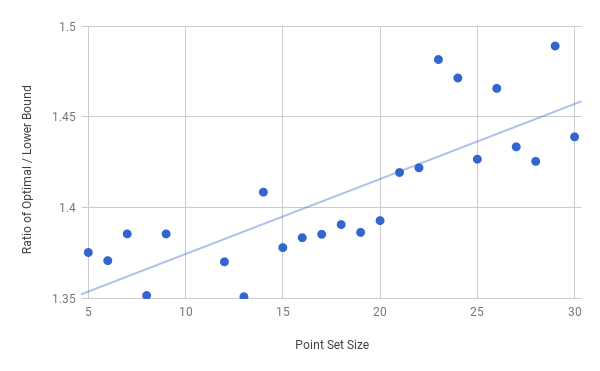
\includegraphics[scale=.38]{lbDivergence}

Fig 2. Increasing divergence between lowerbound and optimal with problem size. The ratio of Optimal Work / Lower Bound Work compared to the point set size fitted with a linear trendline to demonstrate the clear increasing of the ratio with the problem size. Note that two outliers were removed for point set data of size 10 and 11. The values of these were $1.3$ and $1.54$ respectively. 

\section{Results}

In this section, we present the computational results of our algorithm. To determine our algorithm's efficiency, we compare the tours found with it to a few common heuristic approaches. From these results, we acquire a benchmark to measure our algorithm against. Alongside this, we also analyze these results and report on the difference between TBCP tours and TSP tours for different point sets and how much the nature of the TBCP problem statement alters good approximate tours for an instance.

We tested our algorithm on 18 point sets which ranged from 29 points to 9,882 and were acquired from the TSP Test Data at  math.uwaterloo.ca/tsp/data/. As TBCP problems are not symmetric we used 20 different sample start and end points\footnote{The start and end points are the same for each individual sample.} from the datasets and averaged the work and time of the different tests for our results. Our algorithm is then compared to the results of a reverse greedy algorithm, and the Lin-Kernighan TSP algorithm in both unoptimized and optimized form\footnote{The optimization used is Insert-Opt followed by Two-Opt.}. We also compare our algorithm to the reverse greedy algorithm and LK TSP heuristic after they have been optimized by InsertOpt and TwoOpt. The reverse greedy algorithm begins at the starting/ending vertex of the instance and fills in the vertex visited in position $n-1$ with the minimum length edge followed by $n-2$ until a complete tour is formed. The purpose of the reverse nature of this common heuristic is that later position edges in a TBCP effect the amount of work more and therefore should be subject to more minimization. The LK TSP heuristic was found using the Concorde TSP Solver. The instances were solved attempting to minimize distance as a TSP problem. These TSP tours are what is measured against. As the TBCP is asymmetric the minimum of the LK tour and reverse LK tour is used\footnote{Although these tours were generated with the TSP instead of the TBCP in mind, many provide very good solutions to the TBCP due to the minimal distance traveled in the problem. We discuss further on how our algorithm performs against the LK heuristic based on point set characteristics later on.}.

The average runtimes of the TBCP based algorithm, Greedy algorithm, and LK heuristic are shown in Table 1. Although the TBCP algorithm does have a higher runtime on most point sets than the LK heuristic and is much slower than the greedy algorithm, it runs in a reasonable time for all point sets tested. The growth of the algorithm time shows that even for very large point sets, like the last few point sets approaching 10000 points, the TBCP based algorithm can complete execution in under a minute. These numbers also suggest that for point sets larger than 10000, the TBCP algorithm could complete execution in a reasonable amount of time.

The average work of the resulting tours can be seen in Table 2. On average TBCP tours outperformed LK tours by $\%6.4$, optimized LK tours by $\%1.6$, greedy tours by $\%13.5$ and optimized greedy tours by $\%8.3$. For 13 of the 18 runs our TBCP algorithm outperformed the LK heuristic with the best results coming from zi929, outperforming it by $\%24.6$ (Fig 3.). The worst performance of the TBCP vs LK tours came from rw1621, where the TBCP tour was outperformed by $\%5.7$. Our TBCP algorithm performed better than only half of the optimized LK tours with performance ranging from $\%14.1$ better to $\%9.8$ worse than the O-LK tours.

The TBCP algorithm outperformed the unoptimized greedy algorithm on every point set with the highest performance being on dj38 with $\%26.3$ over. Compared to the optimized greedy algorithm the TBCP algorithm outperformed every point set except for ar9152, in which it was outperformed by $\%.7$. These results point towards the idea that the TBCP based algorithm performs better than either of the other two heuristics for TBCPs. It does raise a question, however, about what aspects of a point set promote good algorithm performance compared to other heuristics. This is explored in the next subsection.
\\
\begin{center}
\begin{tabular}{|c|c|c|c|}
 \hline
 \multicolumn{4}{|c|}{Algorithm Runtime Results} \\
 \hline
 Set & TBCP & LK & Greedy\\
 \hline
 w29 & .01 & .01 & .00\\
 \hline
 dj38 & .01 & .01 & .00\\
 \hline
 qa194 & .10 & .11 & .00\\
 \hline
 uy734 & 1.29 & .52 & .00\\
 \hline
 zi929 & .65 & 1.18 & .00\\
 \hline
 lu980 & 1.73 & .60 & .00\\
 \hline
 rw1621 & 5.01 & 1.11 & .01\\
 \hline
 mu1979 & 2.30 & 3.05 & .03\\
 \hline
 nu3496 & 10.26 & 2.31 & .08\\
 \hline
 ca4663 & 14.57 & 4.51 & .13\\
 \hline
 tz6117 & 18.21 & 5.19 & .24\\
 \hline
 eg7146 & 34.13 & 7.34 & .33\\
 \hline
 ym7663 & 29.91 & 8.57 & .38\\
 \hline
 pm8079 & 50.98 & 6.78 & .41\\
 \hline
 ei8246 & 34.47 & 5.43 & .43\\
 \hline
 ar9152 & 41.64 & 8.21 & .53\\
 \hline
 ja9847 & 49.65 & 11.71 & .61\\
 \hline
 gr9882 & 58.82 & 9.45 & .61\\
 \hline
\end{tabular}
\end{center}

Table 1. Average runtime of 20 sample algorithm runs. These values are presented in seconds and calculated by measuring the CPU runtime of the algorithm. The LK results were ran using the Concorde LK solver. Optimization times for LK and Greedy are not included.

\scalebox{.9}{
\begin{tabular}{ |c||c|c|c||c||c|  }
 \hline
 \multicolumn{6}{|c|}{Algorithm Work Results} \\
 \hline
 Set & TBCP & LK & O-LK & Greedy & O-Greedy\\
 \hline
 w29 & 3.41E5 & 3.80E5 & 3.79E5 & 4.21E5 & 4.01E5\\
 \hline
 dj38 & 1.01E5 & 1.15E5 & 1.14E5 & 1.37E5 & 1.34E5\\
 \hline
 qa194 & 6.81E5 & 8.58E5 & 7.93E5 & 8.36E5 & 7.80E5\\
 \hline
 uy734 & 2.74E7 & 2.76E7 & 2.67E7 & 2.97E7 & 2.81E7\\
 \hline
 zi929 & 2.96E7 & 3.93E 7 & 3.43 E 7 & 3.59E7 & 3.37E7\\
 \hline
 lu980 & 5.47E6 & 5.37E6 & 5.22E6 & 5.87E6 & 5.66E6\\
 \hline
 rw1621 & 2.11E7 & 2.00E7 & 1.92E7 & 2.26E7 & 2.19E7\\
 \hline
 mu1979 & 6.76E7 & 7.56E7 & 6.96E7 & 8.93E7 & 7.83E7\\
 \hline
 nu3496 & 1.47E8 & 1.54E8 & 1.48E8 & 1.67E8 & 1.61E8\\
 \hline
 ca4663 & 2.33E9 & 2.59E9 & 2.30E9 & 2.98E9 & 2.62E9\\
 \hline
 tz6117 & 1.07E9 & 1.16E9 & 1.10E9 & 1.35E9 & 1.26E9 \\
 \hline
 eg7146 & 4.47E8 & 5.35E8 & 4.93E8 & 5.23E8 & 4.84E8\\
 \hline
 ym7663 & 7.72E8 & 8.44E8 & 8.04E8 & 8.73E8 & 8.22E8\\
 \hline
 pm8079 & 4.49E8 & 4.43E8 & 4.29E8 & 3.76E8 & 4.60E8\\
 \hline
 ei8246 & 8.81E8 & 8.36E8 & 8.15E8 & 9.27E8 & 8.85E8\\
 \hline
 ar9152 & 3.51E9 & 3.66E9 & 3.47E9 & 3.64E9 & 3.49E9\\
 \hline
 ja9847 & 2.34E9 & 2.37E9 & 2.30E9 & 2.64E9 & 2.49E9\\
 \hline
 gr9882 & 1.44E9 & 1.42E9 & 1.38E9 & 1.62E9 & 1.53E9\\
 \hline
\end{tabular}
}

Table 2. Average work results for 20 sample algorithm runs. These values are the calculated work values for each algorithms run averaged over 20 different uniformly distributed start and end points.

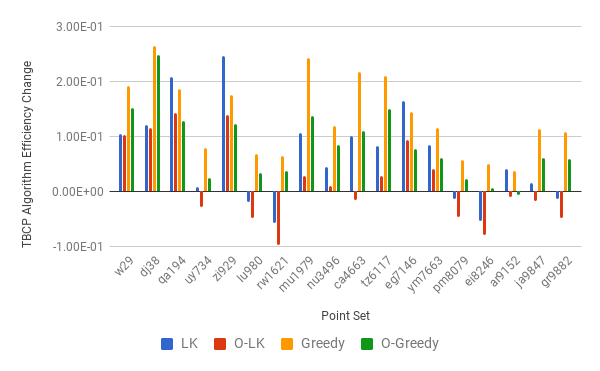
\includegraphics[scale = .38]{TBCPEffeciency}

Fig 3. TBCP algorithm efficiency compared to other heuristic algorithm efficiency. The efficiency was calculated by taking $1 - \frac{W_{TBCP}}{W_{Other}}$ for each algorithm. Work used is the values reported in Table 1.

\subsection{Determining Point Set Specific Efficiency}

As noted in the previous results, different point sets produce very different results from our algorithm compared to the heuristic algorithms we have tested ours against. The most noticeable of these has been the TSP LK heuristic outperforming our TBCP algorithm on some of the point sets. As we do not know the optimal work for any of the TBCP instances, we cannot determine whether this is a result of poor performance of our algorithm on these point sets or good performance of TSP solutions on point sets. Some evidence suggests that it may be due to good TSP solutions. This is because TBCP can in some circumstances have the same optimal solution as the optimal TSP solution. In this subsection, we further explore these relationships and how different aspects of a point set alter them, namely we define a variable $\rho$ which can be used as an estimate of the performance of our algorithm compared to these other common heuristics. 

We gathered a large amount of data on each point set ran, including the distance of the minimum spanning tree of each point set, the average distance to the closest point for each vertex, the range of distances in the point set, the average distance between point in the point set, and the variances of the closest point average and distance average (Table 3). We then looked at these data values to try to determine trends between the data and the efficiency of the TBCP algorithm compared to the Heuristic algorithms. We noticed a slight increase in TBCP efficiency with both closest point variance and distance variance. These correlations strengthened when we too the fraction of variance over the average for these values. Alongside that, we noticed a decrease in efficiency for the TBCP algorithm as the MST grew in size.

Using the observations made above, we came up with the variable $\rho$. The value of $\rho$ is a determination of how much more efficient our algorithm would be than other heuristic choices. Using the correlation between values found above we define $\rho = \frac{\alpha * \frac{\sigma^2_{Distance}}{\mu_{Distance}} + \beta * \frac{\sigma^2_{Closest}}{\mu_{Closest}} - \gamma * \frac{MST}{R}}{R}$, where $\alpha, \beta,$ and $\gamma$ are used to scale how much these values effect $\rho$. By analyzing trendlines for the data, we determined that setting $\alpha = .5, \beta = 6, $ and $\gamma = 14$ gave the best predictive properties to $\rho$. Analyzing the algorithm efficiency compared to this definition of $\rho$, we found a strong upward correlation between the two (Fig 4.). This realization would allow people to determine the usefulness of our algorithm on TBCP point sets prior to running it.\\

\scalebox{.68}{
\begin{tabular}{ |c||c|c|c||c||c| |c| |c|}
 \hline
 \multicolumn{8}{|c|}{Point Set Data} \\
 \hline
 Set & MST & Range & $\mu_{Distance}$ & $\sigma^2_{Distance}$ & $\mu_{Closest}$ & $\sigma^2_{Closest}$ & $\rho$\\
 \hline
 w29 & 21751 & 9564 & 3665 & 4917985 & 573 & 146418 & .227\\
 \hline
 dj38 & 5831 & 1853 & 708 & 149950 & 110 & 8981 & .298\\
 \hline
 qa194 & 8026 & 1458 & 486 & 70277 & 33 & 1286 & .158\\
 \hline
 uy734 & 69874 & 5741 & 2226 & 1147172 & 73 & 2526 & .051 \\
 \hline
 zi929 & 82861 & 7297 & 2547 & 2127820 & 69 & 7463 & .124\\
 \hline
 lu980 & 10205 & 787 & 313 & 24363 & 13 & 35 & -.160 \\
 \hline
 rw1621 & 22973 & 2195 & 733 & 161405 & 20 & 165 & .005\\
 \hline
 mu1979 & 74102 & 10163 & 2844 & 6022496 & 26 & 3048 & .163\\
 \hline
 nu3496 & 84672 & 4928 & 1505 & 956055 & 30 & 764 & .046\\
 \hline
 ca4663 & 1118525 & 90507 & 27944 & 373404522 & 185 & 108578 & .111\\
 \hline
 tz6117 & 347888 & 13698 & 5054 & 6912608 & 44 & 1313 & .037\\
 \hline
 eg7146 & 146700 & 12840 & 2026 & 3278725 & 16 & 1290 & .088\\
 \hline
 ym7663 & 205201 & 12232 & 2507 & 3542792 & 20 & 712 & .056\\
 \hline
 pm8079 & 100465 & 5842 & 1424 & 796929 & 18 & 109 & .012\\
 \hline
 ei8246 & 185256 & 4851 & 1785 & 779507 & 18 & 92 & -.059\\
 \hline
 ar9152 & 741411 & 33201 & 8082 & 26270000 & 93 & 9004 & .057\\
 \hline
 ja9847 & 423471 & 29896 & 7256 & 24579000 & 33 & 1267 & .057\\
 \hline
 gr9882 & 266135 & 10860 & 2935 & 2817774 & 23 & 340 & .021\\
 \hline
\end{tabular}
}

Table 3. Point set data and $\rho$ derivation. The $\rho$ value is obtained from using the formula $\rho = (\alpha * \frac{\sigma^2_{Distance}}{\mu_{Distance}} + \beta * \frac{\sigma^2_{Closest}}{\mu_{Closest}} - \gamma * \frac{MST}{R})/R : \alpha = .5, \beta = 6, \gamma = 14$. This formula is derived as a measurement of the effectiveness of our algorithm compared to other heuristic methods. This relationship is demonstrated in Fig 4.

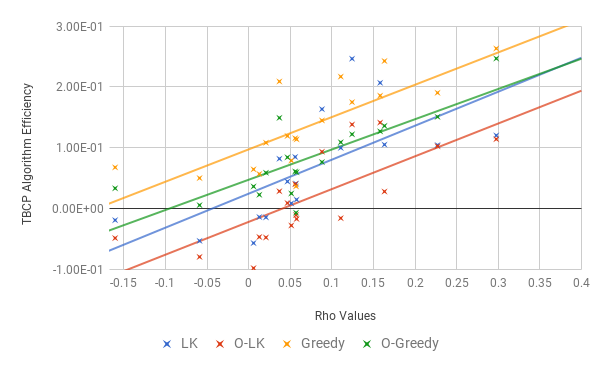
\includegraphics[scale = .38]{rhoValue}

Fig 4. Increasing correlation by TBCP algorithm efficiency and rho values. Each series is comparing the efficiency of the TBCP algorithm vs one common heuristic ($Efficiency = 1 - \frac{W_{TBCP}}{W_{Other}}$) graphed based on $\rho$ values. Linear trendlines have been fitted to the data to demonstrate the clear increasing dependence between the two values.

\section{Conclusion}

This paper has introduced the Tennis Ball Collector Problem as a variation of the Traveling Salesman Problem. For this problem we have presented an algorithm which performs on average better than common heuristic algorithms on TBCP problems, as well as a branch and bound algorithm for small instances of the TBCP and a variation of the TBCP, the C-TBCP. The algorithm presented uses clustering techniques as well as the presented branch and bound technique to find approximate tours through TBCP instances. 

Our algorithm's key aspect is the use of divide and conquer and clustering to break down the complexity of the TBCP. It uses clustering to group vertexes together. These clusters can then be treated as a variation of the TBCP, the C-TBCP, and solved. Given this ordering of clusters, we can then repeat the process on the subproblems within the cluster. This process will give use the tours through each cluster that can then be optimized and finally recombined to make our final tour.

The TBCP has been addressed in terms of both its increased complexity from the TSP as well as the heuristics that can be applied to it. In the result section, we have derived the value $\rho$ for point sets to judge the difference in solutions for the TBCP from the TSP and as a measurement of the usefulness of our algorithm on high $\rho$ sets where other heuristic algorithms may perform poorly.

Although we cannot determine the optimal amount of work for large instances of the TBCP, we tested our algorithm against both the LK and greedy heuristics commonly used for the TSP and showed that on average our algorithm outperforms both of these heuristics. When used along some pointsets, these heuristics can outperform our algorithm but usually by only small percentages whereas the TBCP specific algorithm outperforms them by over $\%20$ in some instances. In future research, these results can be solidified, given a more advanced way to find the minimum work needed for a point set.

The algorithm presented in this paper is just one of many possible heuristic algorithms for TBCP problems. We expect that faster and more effective TBCP specific algorithms can be employed and developed for this problem. Our TBCP algorithm, however, still can be greatly improved. For example, common tour improvement methods can be specialized to the TBCP and implemented in the tour recombination stage of our algorithm. We have also showed briefly that if there is an optimal division of points into clusters, our algorithm is capable of determining the optimal solution for TBCPs. This opens up many avenues to improving its performance based on improved clustering mechanics. This paper lays the groundwork for many possible improvements in approximating near optimal solutions for TBCPs.

\bibliographystyle{alpha}
\bibliography{Bibliography}

\end{document}
